\section{Interface Gráfica}\label{sec:gui}

\FloatBarrier

\begin{figure}[h]
  \centering
  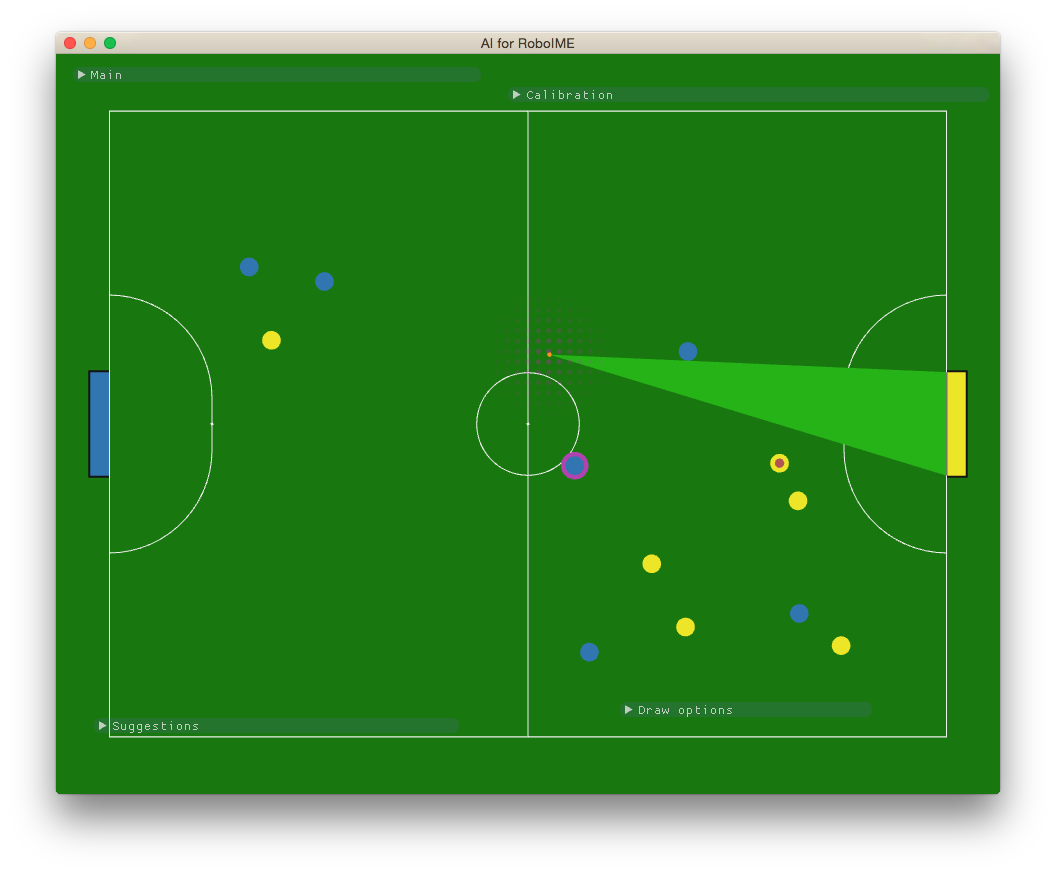
\includegraphics[width=0.8\linewidth]{gui_field}
  \caption{Aparência geral e representação do campo}\label{fig:gui_field}
\end{figure}

A ferramenta representa o estado atual do jogo desenhando o campo, os robôs e a
bola, como pode ser visto na Figura~\ref{fig:gui_field}.  O campo não faz parte
do estado mas é necessário para ter uma referência visual das posições.

\begin{figure}[h]
  \centering
  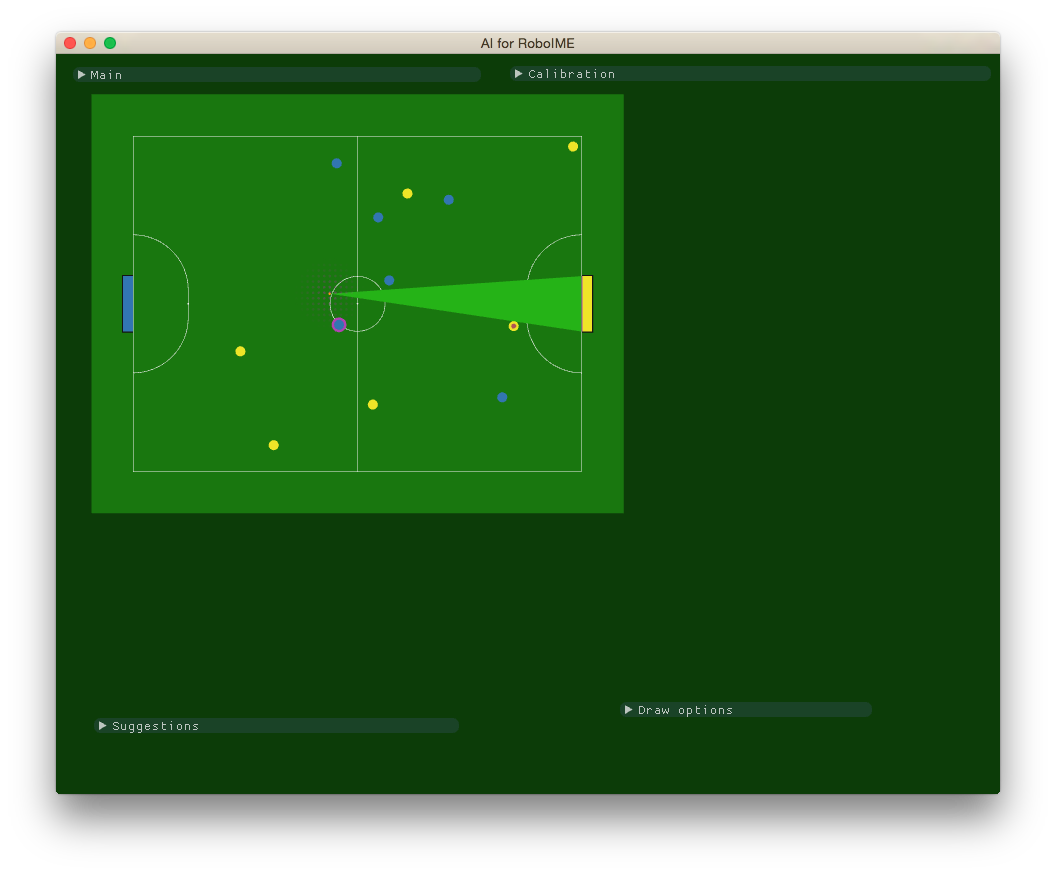
\includegraphics[width=0.4\linewidth]{gui_zoom_out}
  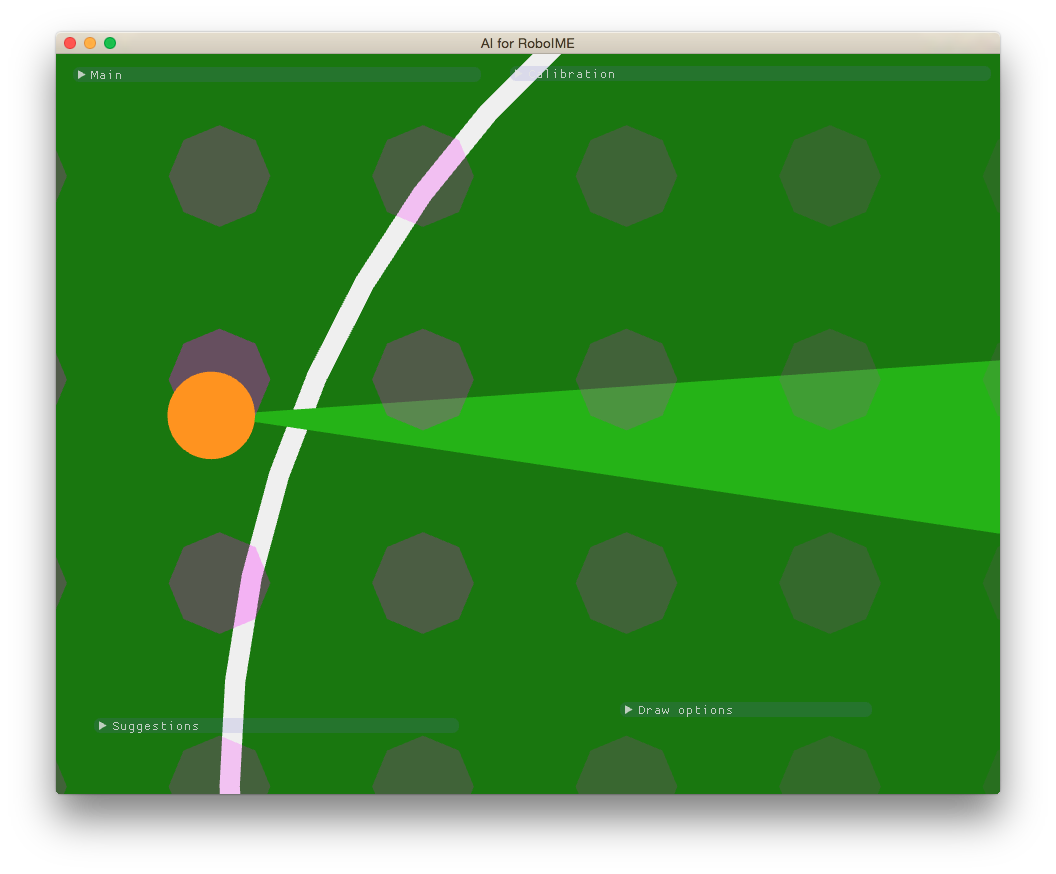
\includegraphics[width=0.4\linewidth]{gui_zoom_in}
  \caption{Zoom e arraste do campo}\label{fig:gui_zoom}
\end{figure}

Para visualizar situações com mais detalhes a ferramenta permite zoom e arraste
do campo (Figura~\ref{fig:gui_zoom}).

\FloatBarrier

\begin{figure}[h]
  \centering
  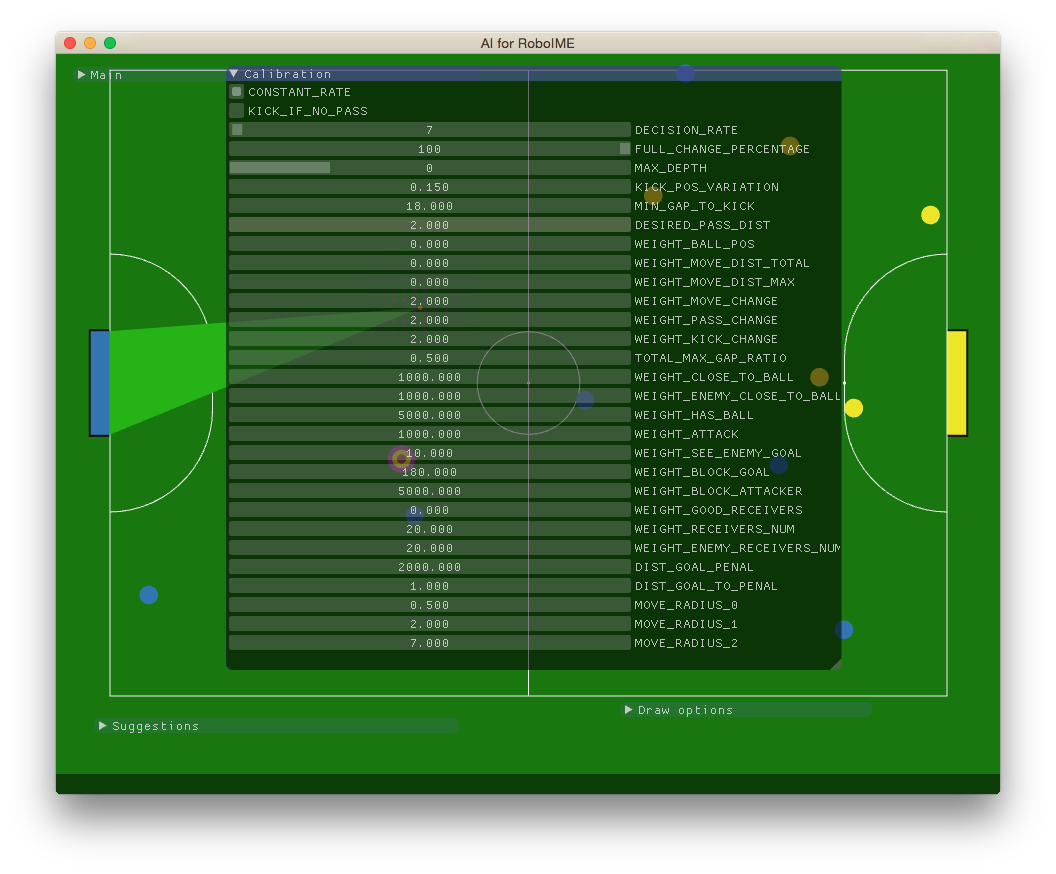
\includegraphics[width=0.75\linewidth]{gui_params}
  \caption{Parâmetros configuráveis}\label{fig:gui_params}
  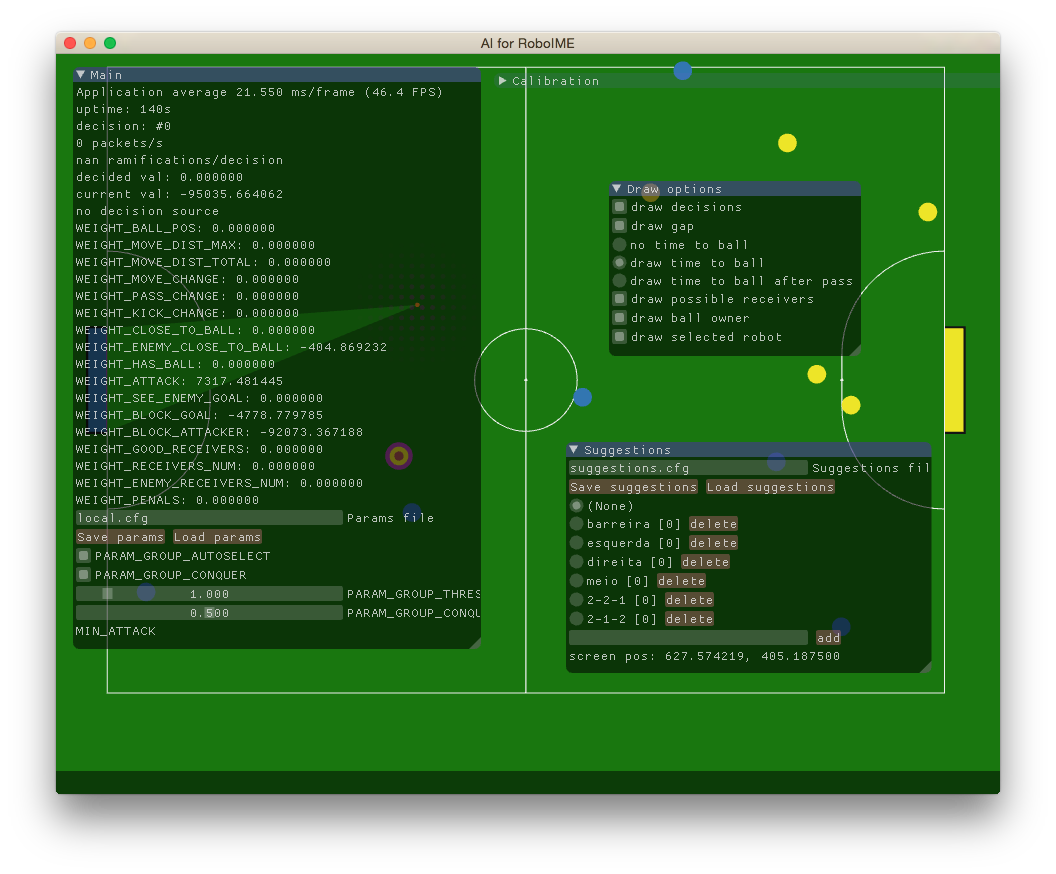
\includegraphics[width=0.75\linewidth]{gui_widgets}
  \caption{Controles}\label{fig:gui_widgets}
\end{figure}

\FloatBarrier

% OBS: "???" em cima das palavras em itálico
Existem quatro abas disponíveis: \textit{Main}, \textit{Calibration},
\textit{Suggestions}, \textit{Draw options}. As abas são retráteis e
translucidas para que as mudanças de configurações possam ser observadas
facilmente.  Na Figura~\ref{fig:gui_field}, por exemplo, todas as estão
minimizadas, na Figura~\ref{fig:gui_params} é mostrada a aba
\textit{Calibration}, as outras três podem ser vistas na
Figura~\ref{fig:gui_widgets}.

\begin{figure}[h]
  \centering
  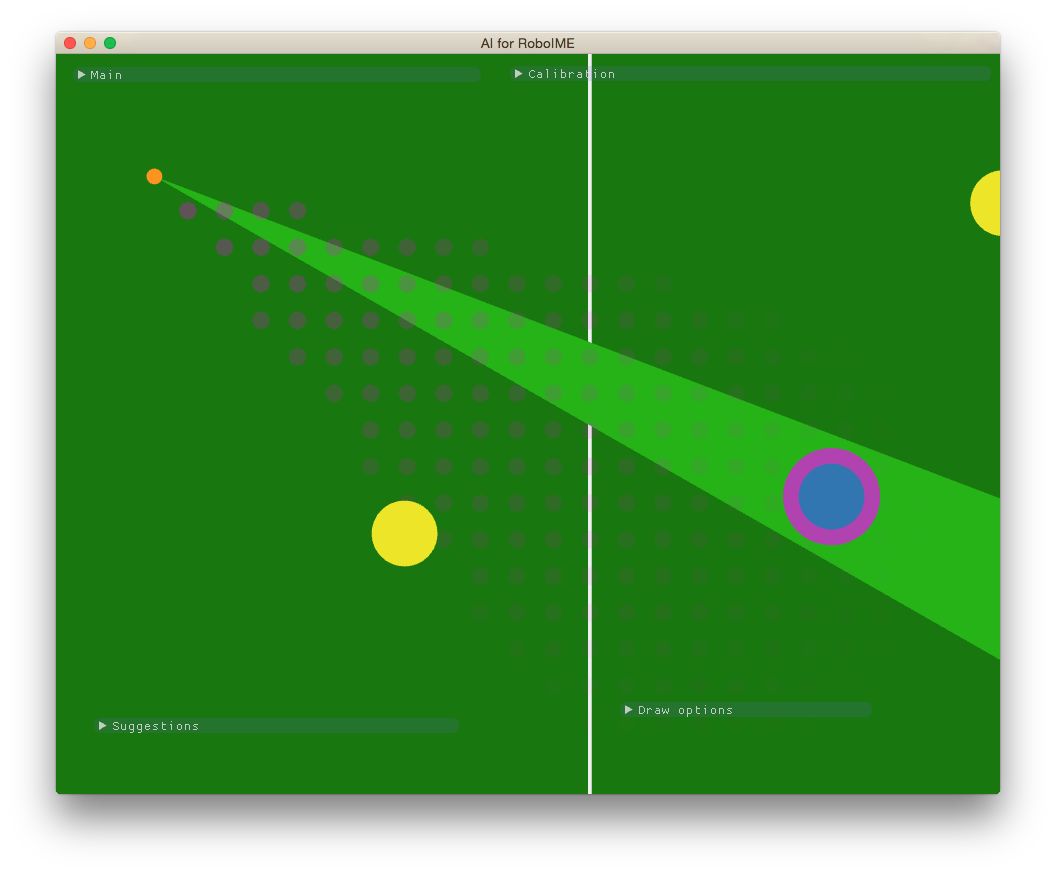
\includegraphics[width=0.4\linewidth]{gui_ball_move}
  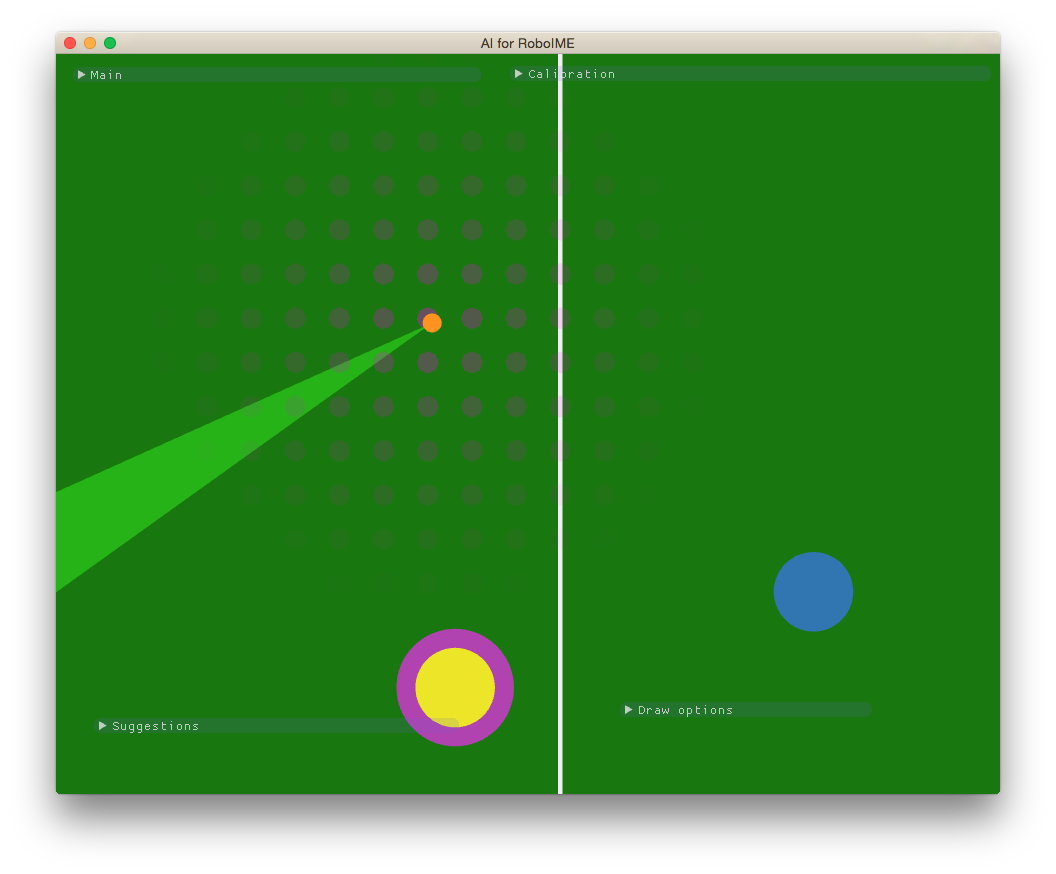
\includegraphics[width=0.4\linewidth]{gui_ball_stop}
  \caption{Representação do tempo para chegar na bola}\label{fig:gui_ball}
\end{figure}

A interface também possui indicadores para o tempo de chegar na bola, o robô que
chegará primeiro na bola e os robôs que podem receber um passe.

O indicador do robô que chegará primeiro, às vezes chamado de "dono da bola", é
representado com um círculo rosa em torno do robô.

O indicador para o tempo de chegar na bola está representado na
Figura~\ref{fig:gui_ball} como um campo de pontos translúcidos ao redor da bola,
quanto maior o diâmetro do ponto menor o tempo para se chegar na bola a partir dali.
% OBS: ele circulou o 'à', mas acho que esta certo
Na imagem à direita, a bola está parada e o robô amarelo é o dono, já na imagem
da esquerda a bola está em movimento, aproximadamente na direção do robô azul,
que nesse caso é o dono da bola.


\begin{figure}[h]
  \centering
  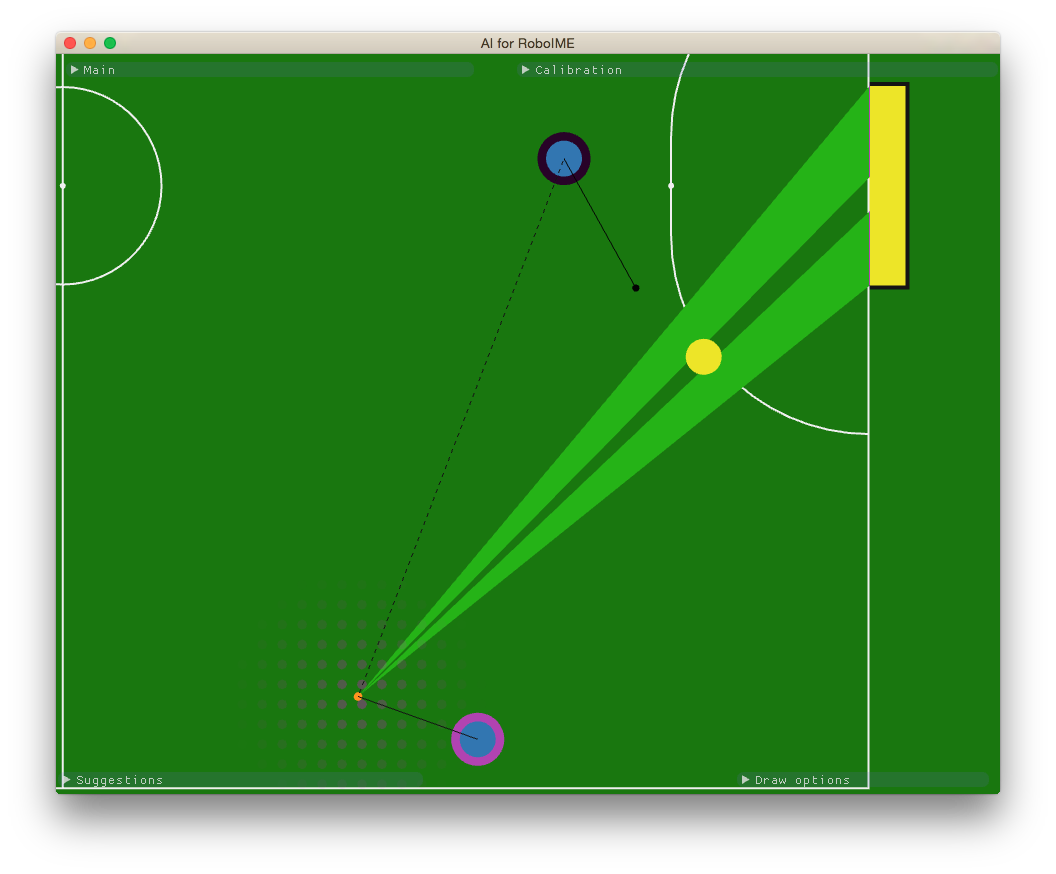
\includegraphics[width=0.8\linewidth]{gui_pass}
  \caption{Representação de ação de passe}\label{fig:gui_pass}
\end{figure}

\begin{figure}[h]
  \centering
  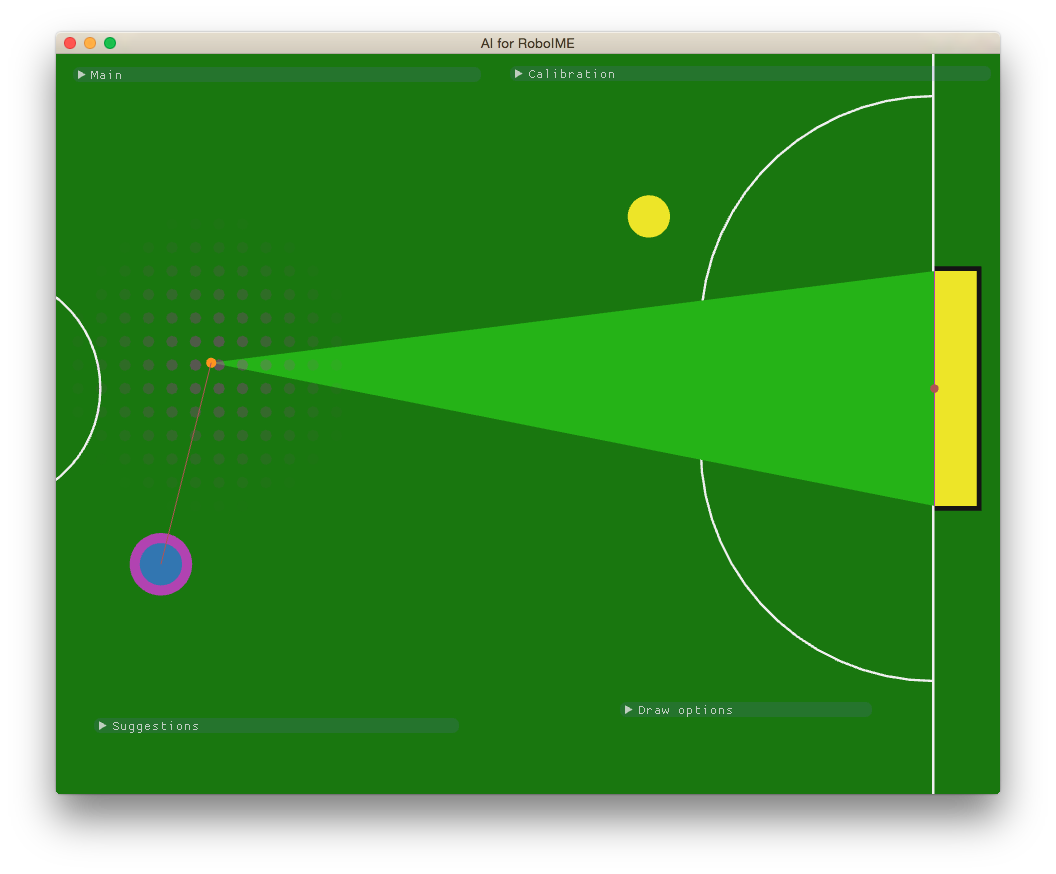
\includegraphics[width=0.8\linewidth]{gui_kick}
  \caption{Representação de ação de chute}\label{fig:gui_kick}
\end{figure}

\begin{figure}[h]
  \centering
  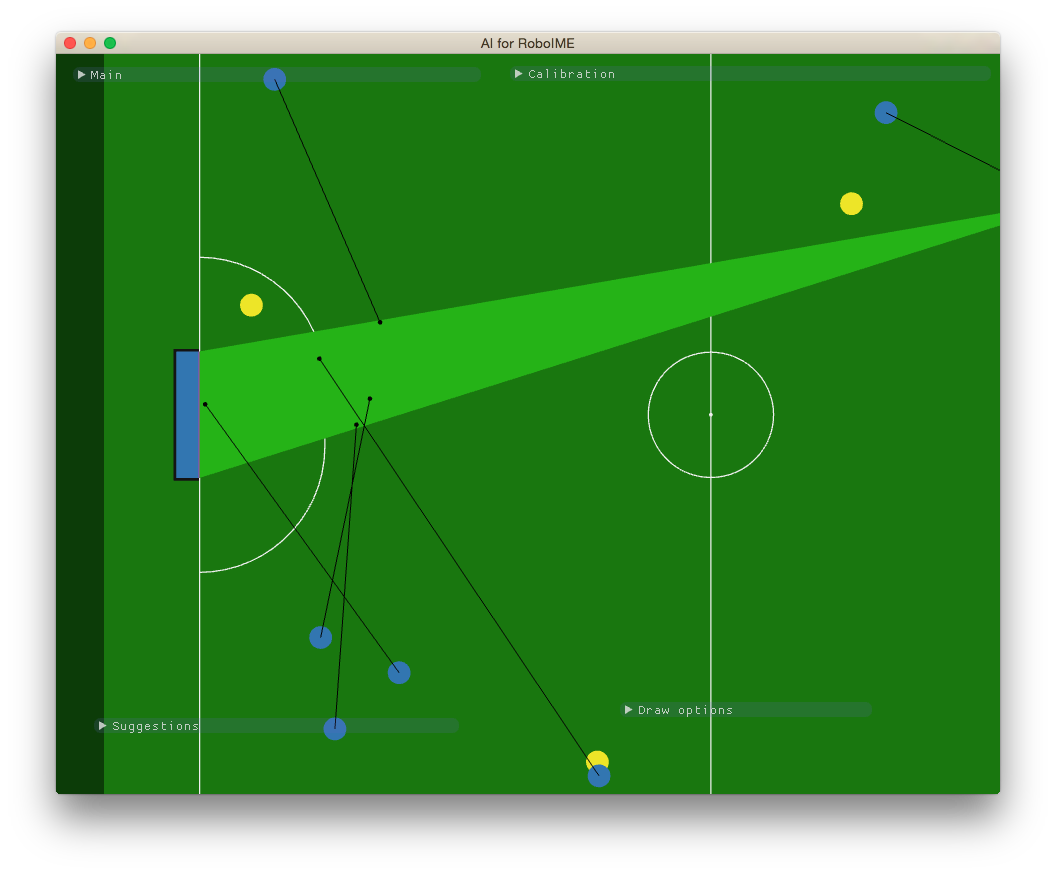
\includegraphics[width=0.8\linewidth]{gui_move}
  \caption{Representação das ações de movimentação}\label{fig:gui_move}
\end{figure}

As decisões tomadas possuem representação gráfica, desenhando individualmente
cada ação.  As ações de passe podem ser vistas na Figura~\ref{fig:gui_pass} uma
linha tracejada da bola para o receptor do passe, nessa mesma figura está
exemplificado a representação dos robôs que podem receber passe.

Similarmente a Figura~\ref{fig:gui_kick} apresenta a representação da ação de
chute.  E por fim, o último tipo de ação e mais comum, a de movimentação, pode
ser vista na Figura~\ref{fig:gui_move}.

\FloatBarrier

% vim: tw=80 et ts=2 sw=2 sts=2 ft=tex spelllang=pt_br,en
